\documentclass{beamer}

\usepackage{graphicx}
\usepackage{framed}
\usepackage{amsmath}
\usepackage{amssymb}
\begin{document}

%==================================================%
%\begin{frame}
% MA4605 2015 Lecture 2B:
% Review of Inference Procedures
% In this class, we shall review some important topics from previous
% modules.
%\end{frame}

\section{Review of Inference Procedures}
%=================================================%
\begin{frame}
	\frametitle{Review of Inference Procedures}
\noindent \textbf{Hypothesis Test}
\begin{itemize}
	\item 	Setting up and testing hypotheses is an essential part of statistics.
	\item In order to formulate such a test, usually some theory has been put
	forward, either because it is believed to be true or because it is to
	be used as a basis for argument, but has not been proved, for
	example, claiming that a new drug is better than the current drug
	for treatment of the same symptoms.
	\item In each problem considered, the question of interest is simplified
	into two competing hypotheses between which we have a choice;
	the null hypothesis, denoted H$_0$, against the alternative hypothesis,
	denoted H$_1$.
\end{itemize}
 
\end{frame}

%=================================================%
\begin{frame}
\frametitle{Hypothesis Tests}
\begin{itemize}
\item These two competing hypotheses are not however treated on an
	equal basis: special consideration is given to the null hypothesis.
\item We have two common situations with regard to formulating hypothesis tests.
\item In the first case, the experiment has been carried out in an attempt to
	disprove or reject a particular hypothesis, the null hypothesis,
	thus we give that one priority so it cannot be rejected unless
	the evidence against it is sufficiently strong.
\end{itemize}
\end{frame}
%=================================================%
\begin{frame}
	For example,
\begin{description}
\item[H$_0$:] there is no difference in taste between Coca Cola and Pepsi
\item[H$_1$:] there is a difference in taste between both.
\end{description}
\end{frame}
%=================================================%
\begin{frame}
\frametitle{Occam's Razor}
\begin{itemize}
	\item If one of the two hypotheses is 'simpler' we give it priority so
	that a more 'complicated' theory is not adopted unless there
	is sufficient evidence against the simpler one.
	\item See Occam's Razor
	\item For example, it is 'simpler' to claim that there is no difference
	in flavour between Coca Cola and Pepsi than it is to say that
	there is a difference.
	\item You would only prefer the more complex claim if there is sufficient evidence to back it up
\end{itemize}

\end{frame}
%=================================================%
\begin{frame}
\noindent \textbf{Testing Parameter values:}
	The hypotheses are often statements about population parameters
	like expected value and variance; for example H$_0$ might be that the
	expected value of the measurements taken by one clinical method
	are different from those of a similar clinical method (assuming both
	methods have the same purpose).
\begin{itemize}
	\item 	A hypothesis might also be a statement about the distributional
	form of a characteristic of interest, for example that clinical
	measurements of a certain quantity are normally distributed.
\item The outcome of a hypothesis test is "Reject H$_0$ in favour of H$_1$" or
	"Do not reject H$_0$".
\end{itemize}

\end{frame}
%=================================================%
\begin{frame}
\frametitle{Null Hypothesis}
	The null hypothesis, H$_0$, represents a theory that has been put
	forward, either because it is believed to be true or because it is to
	be used as a basis for argument, but has not been proved.
	For example, in a clinical trial of a new drug, the null hypothesis
	might be that the new drug is no better, on average, than the
	current drug. We would write
	\begin{description}
		\item[H$_0$:] there is no difference between the two drugs on average.
	\end{description}
	We give special consideration to the null hypothesis. This is due to
	the fact that the null hypothesis relates to the statement being
	tested, whereas the alternative hypothesis relates to the statement
	to be accepted if / when the null is rejected.
	The final conclusion once the test has been carried out is always
	given in terms of the null hypothesis.
\end{frame}
%=================================================%
\begin{frame}
\noindent \textbf{Important:}
\begin{itemize}
	\item 	We either "Reject H$_0$ in favour of H$_1$" or "Do not reject H$_0$".
	We never conclude "Reject H$_1$", or even "Accept H$_1$".
	\item If we conclude "Do not reject H$_0$", this does not necessarily mean
	that the null hypothesis is true, it only suggests that there is not
	sufficient evidence against H$_0$ in favour of H$_1$.
	\item Rejecting the null hypothesis then, suggests that the alternative
	hypothesis may be true.
\end{itemize}

\end{frame}
%=================================================%
\begin{frame}
	\frametitle{Alternative Hypothesis}
\begin{itemize}
	\item 	The alternative hypothesis, H$_1$, is a statement of what a statistical
	hypothesis test is set up to establish.
	\item For example, in a clinical trial
	of a new drug, the alternative hypothesis might be that the new
	drug has a different effect, on average, compared to that of the
	current drug.
	\item We would write
	H$_1$: the two drugs have different effects, on average.
\end{itemize}

\end{frame}
%=================================================%
\begin{frame}
	The alternative hypothesis might also be that the new drug is
	better, on average, than the current drug. In this case we would
	write
	H$_1$: the new drug is better than the current drug, on average.
	The final conclusion once the test has been carried out is always
	given in terms of the null hypothesis. As before, we either "Reject
	H$_0$ in favour of H$_1$" or "Do not reject H$_0$".
	We never conclude "Reject H$_1$", or even "Accept H$_1$".
	If we conclude "Do not reject H$_0$", this does not necessarily mean
	that the null hypothesis is true, it only suggests that there is not
	sufficient evidence against H$_0$ in favour of H$_1$.
	Rejecting the null hypothesis then, suggests that the alternative
	hypothesis may be true.
\end{frame}
\section{Confidence Intervals}
%=================================================%
\begin{frame}
	\frametitle{Confidence Intervals}
\textbf{Confidence Interval}
\begin{itemize}
\item 	A confidence interval gives an estimated range of values which is
		likely to include an unknown population parameter, the estimated
		range being calculated from a given set of sample data.
\item If independent samples are taken repeatedly from the same
		population, and a confidence interval calculated for each sample,
		then a certain percentage (confidence level) of the intervals will
		include the unknown population parameter.
\item Confidence intervals are usually calculated so that this percentage is
		95\%, but we can produce 90\%, 99\%, 99.9\% (or whatever)
		confidence intervals for the unknown parameter.
\end{itemize}

\end{frame}
%=================================================%
\begin{frame}
\begin{itemize}
\item 	The width of the confidence interval gives us some idea about how
	uncertain we are about the unknown parameter (recall precision). 
\item A
	very wide interval may indicate that more data should be collected
	before anything very definite can be said about the parameter.
\item Confidence intervals are more informative than the simple results of
	hypothesis tests (where we decide "reject H$_0$" or "don't reject H$_0$")
	since they provide a range of plausible values for the unknown
	parameter.
\end{itemize}

\end{frame}
\section{Confidence Limits}
%=================================================%
\begin{frame}
\frametitle{Confidence Limits}
	Confidence limits are the lower and upper boundaries / values of a
	confidence interval, that is, the values which define the range of a
	confidence interval.
	The upper and lower bounds of a 95\% confidence interval are the
	95\% confidence limits. These limits may be taken for other
	confidence levels, for example, 90\%, 99\%, 99.9\%.

\end{frame}
\section{Confidence Level}
%=================================================%
\begin{frame}
\begin{itemize}
	\item 	The confidence level is the probability value ($1-\alpha$) associated with a
	confidence interval.
	It is often expressed as a percentage.
	For example, say $\alpha = 0.05 = 5\%$, then the confidence level is equal
	to (1-0.05) = 0.95, i.e. a 95\% confidence level.
\end{itemize}


\end{frame}

\section{Significance Level}
%=================================================%
\begin{frame}
\frametitle{Significance Level}	
	The significance level of a statistical hypothesis test is a fixed
	probability of wrongly rejecting the null hypothesis H$_0$, if it is in fact
	true.
\end{frame}
%=================================================%
\begin{frame}It is the probability of a type I error and is set by the investigator
	in relation to the consequences of such an error. That is, we want to
	make the significance level as small as possible in order to protect
	the null hypothesis and to prevent, as far as possible, the
	investigator from inadvertently making false claims.
	The significance level is usually denoted by $\alpha$
	\[Significance Level = P(type I error) =\alpha\]
	Usually, the significance level is chosen to be 0.05 (i.e. 5%).
\end{frame}
\section{Outcomes of Hypothesis Tests}
%=================================================%
\begin{frame}	
\frametitle{Test Statistic}
	A test statistic is a quantity calculated from our sample of data. Its
	value is used to decide whether or not the null hypothesis should be
	rejected in our hypothesis test.
	The choice of a test statistic will depend on the assumed probability
	model and the hypotheses under question.

\end{frame}
%=================================================%
\begin{frame}
\frametitle{P-Value}
	The probability value (p-value) of a statistical hypothesis test is the
	probability of getting a value of the test statistic as extreme as or
	more extreme than that observed by chance alone, if the null
	hypothesis H$_0$, is true.
	It is the probability of wrongly rejecting the null hypothesis if it is in
	fact true.
\end{frame}
%=================================================%
\begin{frame}
		It is equal to the significance level of the test for which we would
	only just reject the null hypothesis.
	The p-value is compared with the actual significance level of our
	test and, if it is smaller, the result is significant. That is, if the null
	hypothesis were to be rejected at the 5\% significance level, this
	would be reported as "p < 0.05".
\end{frame}
%=================================================%
\begin{frame}	Small p-values suggest that the null hypothesis is unlikely to be
	true. The smaller it is, the more convincing is the rejection of the
	null hypothesis.
	It indicates the strength of evidence for say, rejecting the null
	hypothesis H$_0$, rather than simply concluding "Reject H$_0$' or "Do not
	reject H$_0$".
	When using R, we will see a classification structure for various
	levels of p-values.
\end{frame}

	\section{Type I and II Errors, and Power}
	
	%============================================================%
	\begin{frame}
		\frametitle{Type I and II Error}
		\large
		\begin{itemize}
			\item In a hypothesis test, a type I error occurs when the null hypothesis
			is rejected when it is in fact true; that is, H0 is wrongly rejected.
			For example, in a clinical trial of a new drug, the null hypothesis
			might be that the new drug is no better, on average, than the
			current drug; i.e.
		\end{itemize}
			\begin{description}
				\item[H0: ] there is no difference between the two drugs on average.
			\end{description}
\end{frame}
%============================================================%
\begin{frame}
			\frametitle{Type I and II Error}
			\large
			\noindent \textbf{Type I Errors}
			\begin{itemize}
				\item A type I error would occur if we concluded that the two drugs
				produced different effects when in fact there was no difference
				between them.
				
				
				\item The hypothesis test procedure is therefore adjusted so that there is
				a guaranteed 'low' probability of rejecting the null hypothesis
				wrongly; this probability is never 0.
				
				\item This probability of a type I error can be precisely computed as
				\[\Pr(\mbox{type I error}) = \mbox{significance level} = \alpha\]
				
			\end{itemize}
\end{frame}
%============================================================%
\begin{frame}
\frametitle{Type I and II Error}
\large
\begin{itemize}
				\item For any given set of data, type I and type II errors are inversely
				related; the smaller the risk of one, the higher the risk of the other.
				\item A type I error can also be referred to as an error of the first kind.
			\end{itemize}
			Type II Error
			\begin{itemize}
				\item In a hypothesis test, a type II error occurs when the null hypothesis
				H0, is not rejected when it is in fact false. 
				\item For example, in a clinical
				trial of a new drug, the null hypothesis might be that the new drug
				is no better, on average, than the current drug; i.e.
				H0: there is no difference between the two drugs on average.
			\end{itemize}
			
\end{frame}
%============================================================%
\begin{frame}
			\frametitle{Type II Error}
			\large
			\begin{itemize}
				\item A type II error would occur if it was concluded that the two drugs
				produced the same effect, i.e. there is no difference between the
				two drugs on average, when in fact they produced different ones.
				A type II error is frequently due to sample sizes being too small.
				\item The probability of a type II error is generally unknown, but is
				symbolised by β and written
				\[P(\mbox{type II error}) = \beta\]
				\item A type II error can also be referred to as an error of the second
				kind.
				\item The exact probability of a type II error is generally unknown.
				If we do not reject the null hypothesis, it may still be false (a type
				II error) as the sample may not be big enough to identify the
				falseness of the null hypothesis (especially if the truth is very close
				to hypothesis).
			\end{itemize}
		\end{frame}
%============================================================%
\begin{frame}
			\frametitle{Review of Inference Procedures}
			\large
			
			\textbf{Summary:}\\
			The following table gives a summary of possible results of any
			hypothesis test:
			\begin{figure}
				\centering
				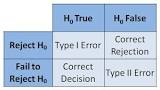
\includegraphics[width=0.6\linewidth]{ErrorTypeTable}
				
			\end{figure}
			
			
\end{frame}
%============================================================%
\begin{frame}
\frametitle{Type I and II Error}
\large
\begin{itemize}
\item A type I error is often considered to be more serious, and therefore
				more important to avoid, than a type II error. 
\end{itemize}
\textbf{Power}
\begin{itemize}
\item The power of a statistical hypothesis test measures the test's ability
to reject the null hypothesis when it is actually false - that is, to
make a correct decision.
\end{itemize}
\end{frame}
%============================================================%
\begin{frame}
\frametitle{Review of Inference Procedures}
\large
\begin{itemize}
\item In other words, the power of a hypothesis test is the probability of
				not committing a type II error. 
\item It is calculated by subtracting the
				probability of a type II error from 1, usually expressed as:
				\[Power = 1 - P(\mbox{type II error}) = 1- \beta\]
\item The maximum power a test can have is 1, the minimum is 0. Ideally
				we want a test to have high power, close to 1.
\end{itemize}
\end{frame}
\section{One Tailed Testing}
%============================================================%

\begin{frame}
\frametitle{Review of Inference Procedures}
\large
\noindent \textbf{One Tailed Testing}
\begin{itemize}
				\item A one-sided test is a statistical hypothesis test in which the values
				for which we can reject the null hypothesis, H0 are located entirely
				in one tail of the probability distribution.
				\item In other words, the critical region for a one-sided test is the set of
				values less than the critical value of the test, or the set of values
				greater than the critical value of the test.
\end{itemize}
			
			
\end{frame}
%============================================================%
\begin{frame}
			\frametitle{Review of Inference Procedures}
			\large
			\begin{itemize}
				\item We generally use it to formally test whether a parameter value is
				greater or less than some specified value, or for the case of two
				samples, if the parameter values from sample is greater or less
				than the corresponding parameter value from the other sample.
				\item A one-sided test is also referred to as a one-tailed test of
				significance.
				\item Remark: For the sake of brevity, we will mostly work on the basis of two-tailed tests throughout this module.
				\item The choice between a one-sided and a two-sided test is determined
				by the purpose of the investigation or prior reasons for using a onesided
				test.
			\end{itemize}
			
			
		\end{frame}

\section{One Sample Procedures}
%=================================================%
\begin{frame}
	\frametitle{One Sample t-test}
	A one sample t-test is a hypothesis test for answering questions
	about the mean where the data are a random sample of
	independent observations from an underlying normal distribution
	$N(\mu,\sigma^2 )$, where is unknown.
	The null hypothesis for the one sample t-test is:
	H$_0$: $\mu = \mu_0$, where $\mu_0$ is some specified number.
	That is, the sample has been drawn from a population of given
	mean and unknown variance (which therefore has to be estimated
	from the sample).
	This null hypothesis, H$_0$ is tested against one of the following
	alternative hypotheses, depending on the question posed:
	\begin{description}
		\item[H$_1$:] $\mu$ is not equal to $\mu_0$
		\item[H$_1$:] $\mu > \mu_0$
		\item[H$_1$:] $\mu < \mu_0$
	\end{description}	
\end{frame}
%=================================================%
\begin{frame}
	\frametitle{Confidence Interval for a Mean}
	A confidence interval for a mean specifies a range of values within
	which the unknown population parameter, in this case the mean,
	may lie. These intervals may be calculated by, for example, a
	medical researcher who wishes to estimate the mean response by
	patients to a new drug; etc.
\end{frame}
%=================================================%
\begin{frame}
	\frametitle{Confidence Interval for a Mean}	
	The (two sided) confidence interval for a mean contains all the
	values of $\mu_0$ (the true population mean) which would not be
	rejected in the two-sided hypothesis test of:
	H$_0$: $\mu = \mu_0$
	H$_1$: $\mu$ not equal to $\mu_0$
	The width of the confidence interval gives us some idea about how
	uncertain we are about the unknown population parameter, in this
	case the mean.
\end{frame}
%=================================================%
\begin{frame}
	\frametitle{Confidence Intervals}
	\begin{itemize}
		\item 	A very wide interval may indicate that more data should be
		collected before anything very definite can be said about the
		parameter.
		
		We calculate these intervals for different confidence levels,
		depending on how precise we want to be. We interpret an interval
		calculated at a 95\% level as “we are 95\% confident that the interval
		contains the true population mean”.
		We could also say that 95\% of all confidence intervals formed in
		this manner (from different samples of the population) will include
		the true population mean.
	\end{itemize}
	
	
\end{frame}

\section{Two Sample Procedures}
%=================================================%
\begin{frame}
	\frametitle{Two Sample t-test}
	A two sample t-test is a hypothesis test for answering questions
	about the mean where the data are collected from two random
	samples of independent observations, each from an underlying
	normal distribution:
	Important: When carrying out a two sample t-test, it is common to
	assume that the variances for the two populations are equal, i.e.
	The null hypothesis for the two sample t-test is:
	H$_0$: $\mu_1 = \mu_2$
	That is, the two samples have both been drawn from the same
	population. 
\end{frame}

\section{Two Sample Procedures}
%=================================================%
\begin{frame}
	\frametitle{Two Sample t-test}
	This null hypothesis is tested against one of the
	following alternative hypotheses, depending on the question posed.
	H$_1$: $\mu_1$ is not equal to $\mu_2$
	H$_1$: $\mu_1 > \mu_2$
	H$_1$: $\mu_1 < \mu_2$
\end{frame}
%=================================================%
\begin{frame}
	\noindent \textbf{Confidence Interval for the Difference Between Two Means}
	\begin{itemize}
		\item 	A confidence interval for the difference between two means
		specifies a range of values within which the difference between the
		means of the two populations may lie.
		\item These intervals may be calculated by, for example, a medical
		researcher who wishes to estimate the difference in mean response
		by patients who are receiving two different drugs; etc.
	\end{itemize}
\end{frame}
%=================================================%
\begin{frame}
	\noindent \textbf{The confidence interval for the difference between two means}
	
	\begin{itemize}
		\item This interval	contains all the values of $\mu_1 - \mu_2$ (the difference between the two
		population means) which would not be rejected in the two-sided
		hypothesis test of:
	\end{itemize}
	\begin{description}
		\item[H$_0$:] $\mu_1 = \mu_2$
		\\against
		\item[H$_1$:] $\mu_1$ not equal to $\mu_2$
	\end{description}
	
	Equivalently
	\begin{description}
		\item[H$_0$:] $\mu_1 - \mu_2 = 0$
		\\against
		\item[H$_1$:] $\mu_1 - \mu_2$ not equal to 0
	\end{description}
	
\end{frame}
%=================================================%
\begin{frame}Important:
	\begin{itemize}
		\item 	If the confidence interval includes 0 we can say that there is no
		significant difference between the means of the two populations, at
		a given level of confidence.
		interpret an interval calculated at a 95\% level as ”\textit{we are 95\%
			confident that the interval contains the true difference between the
			two population means}”. 
		\item We could also say that 95\% of all
		confidence intervals formed in this manner (from different samples
		of the population) will include the true difference.
	\end{itemize}
\end{frame}
\section{Paired T Test}
	%============================================================%
\begin{frame}
\frametitle{Review of Inference Procedures}
\large
\noindent \textbf{Paired t-test}
A paired t-test is used to compare two population means where
there are two samples in which observations in one sample can be
paired with observations in the other sample.\\ \smallskip
			Examples of where this might occur are:
			\begin{itemize}
				\item Before-and-after observations on the same subjects (e.g.
				patient’s diagnostic test results before and after a particular
				course of treatment).
				\item A comparison of two different methods of measurement or
				two different treatments where the measurements/treatments
				are applied to the same subjects (e.g. measurements made
				with Ultra Violet Spectroscopy and Near Infrared Reflectance
				spectroscopy).
\end{itemize}
			
			
\end{frame}
%============================================================%
\begin{frame}
\frametitle{Review of Inference Procedures}
			\large
			The hypotheses can be stated as follows:
			\begin{description}
				\item[H0:] $mu_{diff} =0$ Population mean of case-wise differences is zero
				\item[H1:] $mu_{diff} =0$\label{$mu_{diff}$ ≠ 0} Population mean of case-wise differences is not zero
			\end{description}
			\begin{itemize}
				\item The null hypothesis would articulate the argument that a course of
				treatment had no effect on the subjects, or for the second case,
				that there is no significant measurement bias between two methods
				of measurement.
				\item We will perform a case study of this in the Lab Classes.
			\end{itemize}
		\end{frame}
		%============================================================%
	\end{document}

